\begin{frame}
	\myheading{Module 12.5 : YOLO model for object detection}
\end{frame}

%%%%%%%%%%%%%%%%%%%%%%%%%%%%%%%%%%%%%%%%%%%%%%%%%%%%%%%%%%%%%%%%%%%%%%%%%%%%%%

\begin{frame}
	\begin{columns}
		\column{0.5\textwidth}
		\begin{overlayarea}{\textwidth}{\textheight}
			\begin{tikzpicture}
	\onslide<1->{
		\node (img){
			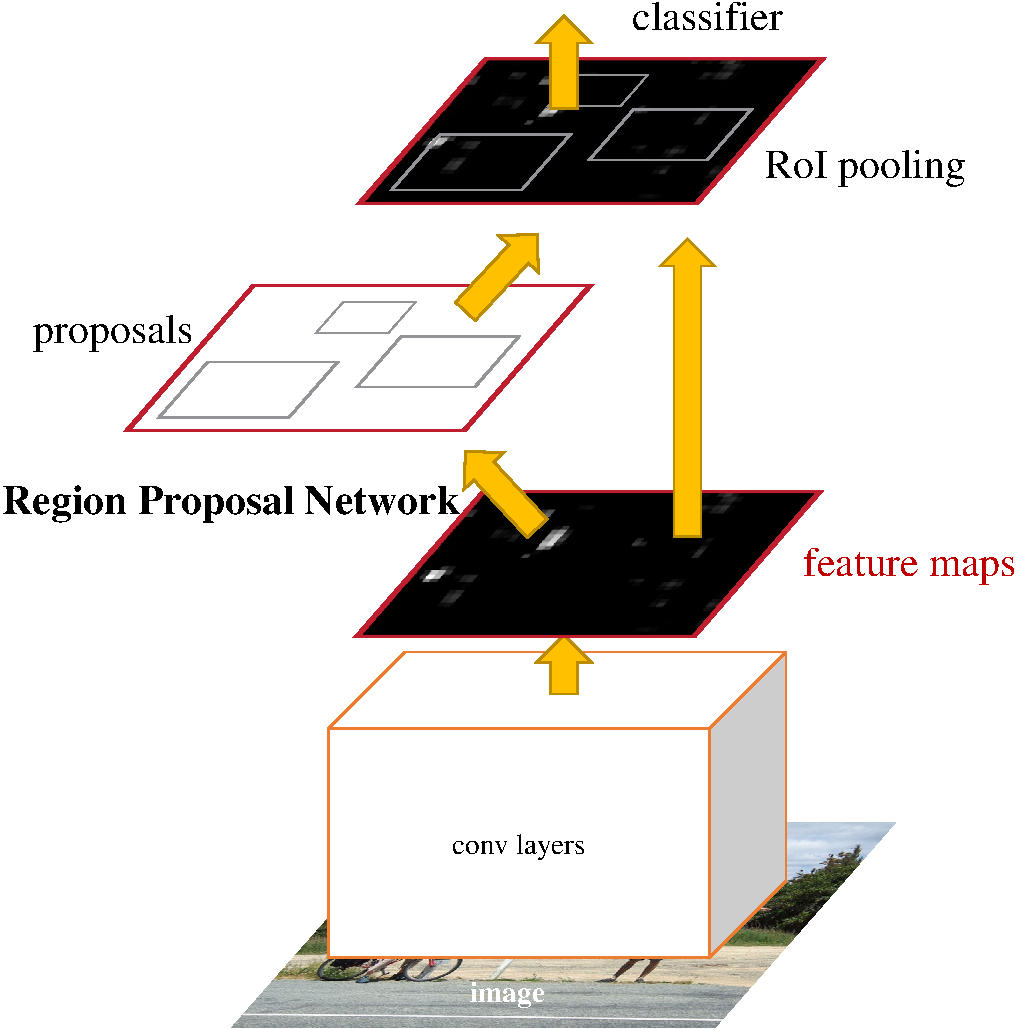
\includegraphics[width=1.0\linewidth]{images/model}
		};    
	}

	\onslide<2,4->{
		\draw[->,line width=1.5mm,color=green!50!white](-3,-1)--(-1,0);   
	}


	\onslide<3->{
		\draw[->,line width=1.5mm,color=red!50!white](-3,4)--(-1,3);    
	}   
\end{tikzpicture}

		\end{overlayarea}     
		\column{0.5\textwidth}
		\begin{overlayarea}{\textwidth}{\textheight}    
			\begin{itemize}
				\justifying
				\onslide<1->{\item The approaches that we have seen so far are two stage approaches }
				\onslide<2->{\item They involve a region proposal stage and then a classification stage }
				\onslide<4->{\item Can we have an end-to-end architecture which does both proposal and classification simultaneously ?}
				\onslide<5->{\item This is the idea behind \textbf{YOLO-}You Only Look Once. }
			\end{itemize}
		\end{overlayarea}
	\end{columns}
	
\end{frame}

%%%%%%%%%%%%%%%%%%%%%%%%%%%%%%%%%%%%%%%%%%%%%%%%%%%%%%%%%%%%%%%%%%%%%%%%%%%%%%

\begin{frame}
	\begin{overlayarea}{\textwidth}{\textheight}  
		\begin{columns}
			\column{0.5\textwidth}
			\vspace*{0.3\linewidth}
			\begin{tikzpicture}
	\centering
	
	\draw (0,0) grid[xstep=0.5,ystep=0.5] (5,0.5);
	\node (w) at (0.25,0.25) {\scriptsize $c$};
	\node (h) at (0.75,0.25) {\scriptsize $w$};
	\node (x) at (1.25,0.25) {\scriptsize $h$};
	\node (y) at (1.75,0.25) {\scriptsize $x$};
	\node (pc) at (2.25,0.25) {\scriptsize $y$};
	\node (pd) at (2.75,0.75) {\scriptsize $P(cow)$};

	\node (w) at (3.25,-0.25) {\scriptsize $P(dog)$};
	\node (h) at (3.75,0.25) {$\cdot$};

	\node (w) at (4.25,0.25) {$\cdot$};
	\node (h) at (4.75,0.75) {\scriptsize $P(truck)$};



	\node(img) at (2.5,-3){
		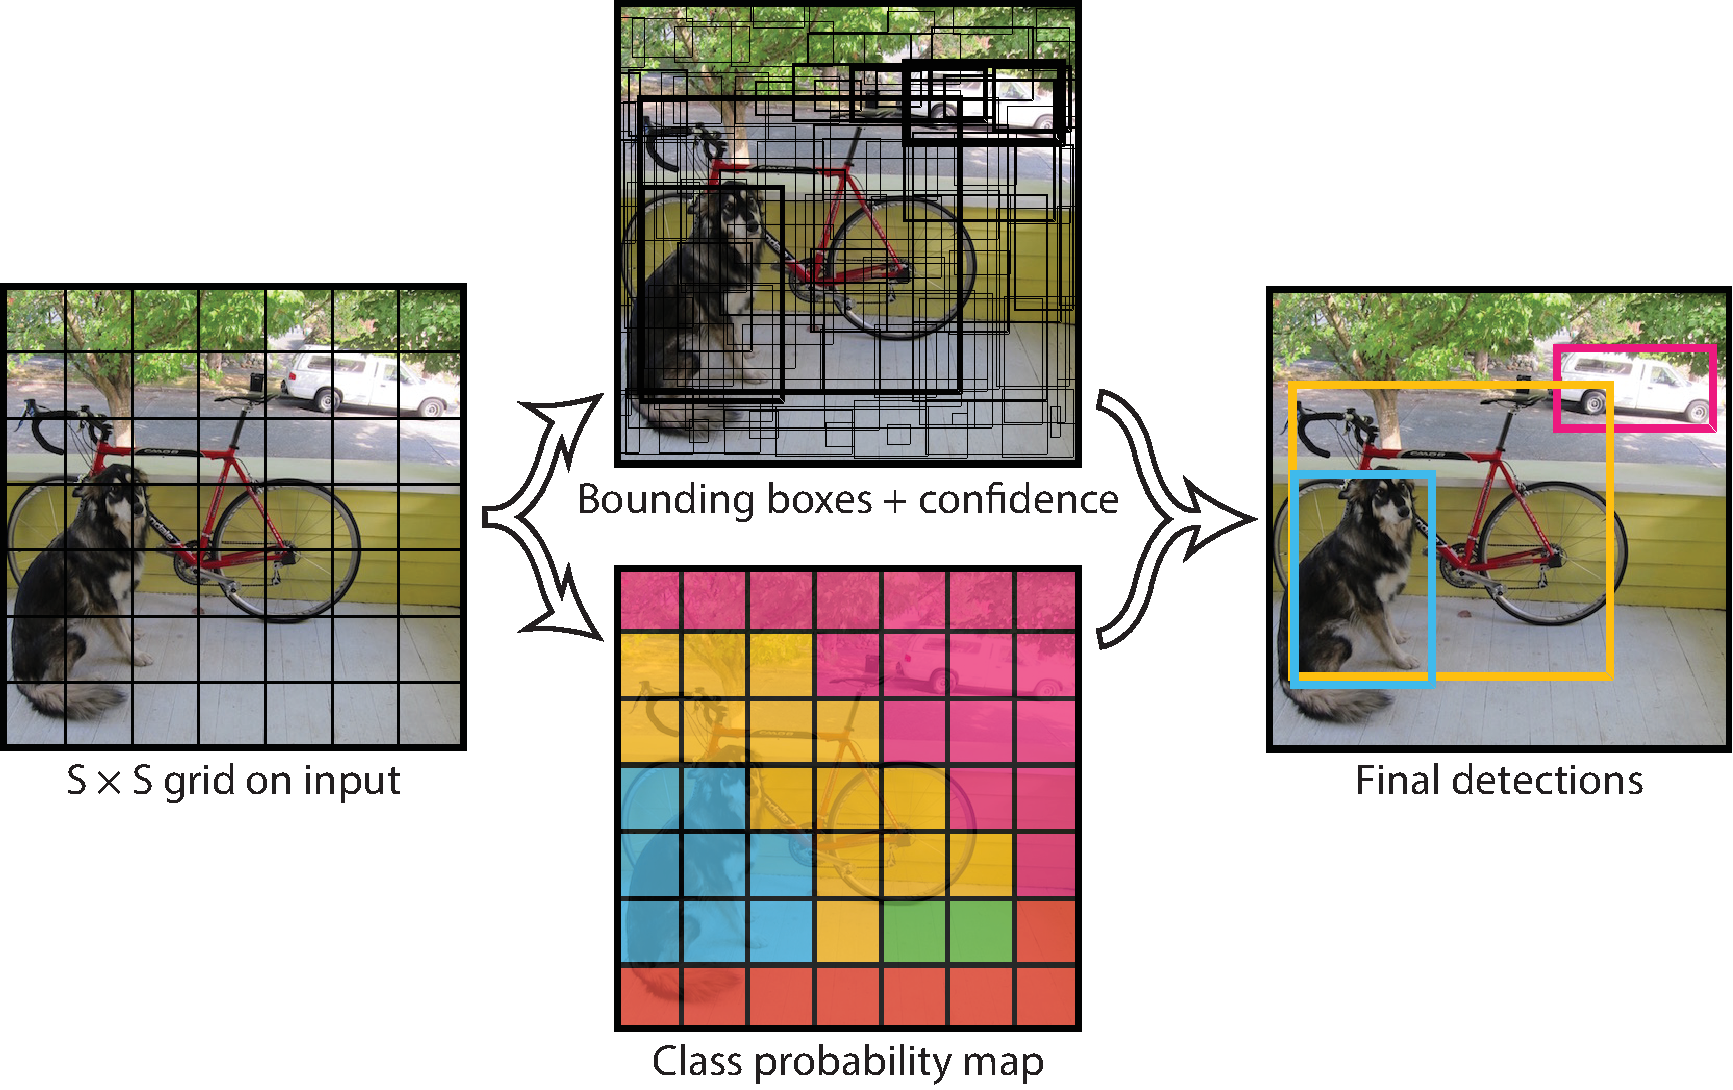
\includegraphics[scale=0.4,trim={0cm 4.5cm 21.2cm 4cm},clip]{images/dog.pdf}
	};


	\draw (0,0) grid[xstep=0.5,ystep=0.5] (5,0.5);

	\onslide<2->{
		\pgfmathsetmacro\x{1.3}
		\pgfmathsetmacro\y{-3.6}
		\filldraw[fill=red!30!white, draw=black,opacity=0.6](\x,\y) rectangle (\x+0.5,\y+0.5);    
	}
	
	\only<3>{
		\filldraw[fill=green!40!white, draw=black](0,0) rectangle (0.5,0.5);    
		\node (w) at (0.25,0.25) {\scriptsize $c$};
	}

	\only<4>{
		\filldraw[fill=green!40!white, draw=black](0.5,0) rectangle (1,0.5);    
		\node (h) at (0.75,0.25) {\scriptsize $w$};
	}

	\only<5>{
		\filldraw[fill=green!40!white, draw=black](1,0) rectangle (1.5,0.5);    
		\node (x) at (1.25,0.25) {\scriptsize $h$};
	} 
	
	\only<6>{
		\filldraw[fill=green!40!white, draw=black](1.5,0) rectangle (2,0.5);    
		\node (y) at (1.75,0.25) {\scriptsize $x$};
		\filldraw[fill=green!40!white, draw=black](2,0) rectangle (2.5,0.5);    
		\node (x) at (2.25,0.25) {\scriptsize $y$};
	} 

	\onslide<7->{

		\filldraw[fill=green!40!white, draw=black](2.5,0) rectangle (5,0.5);
		\draw (0,0) grid[xstep=0.5,ystep=0.5] (5,0.5);
		\node (pd) at (2.75,0.75) {\scriptsize $P(cow)$};

		\node (w) at (3.25,-0.25) {\scriptsize $P(dog)$};
		\node (h) at (3.75,0.25) {$\cdot$};

		\node (w) at (4.25,0.25) {$\cdot$};
		\node (h) at (4.75,0.75) {\scriptsize $P(truck)$};
	}   
\end{tikzpicture}
			\column{0.5\textwidth}
			\begin{overlayarea}{\textwidth}{\textheight}
				\begin{itemize}
					\justifying
					\onslide<1->{\item Divide an image into $S \times S$ grids (S=7)}
					\onslide<2->{\item For each such cell we are interested in predicting $5+k$ quantities}
					\onslide<3->{\item Probability (confidence) that this cell is indeed contained in a true bounding box}
					\onslide<4->{\item Width of the bounding box}
					\onslide<5->{\item Height of the bounding box}
					\onslide<6->{\item Center (x,y) of the bounding box}
					\onslide<7->{\item Probability of the object in the bounding box belonging to the $k^{th}$ class (k - values)}
					\onslide<8->{\item The output layer thus contains $S \times S \times (5+k)$ elements}
				\end{itemize}
				
			\end{overlayarea}
		\end{columns}
	\end{overlayarea}
\end{frame}

%%%%%%%%%%%%%%%%%%%%%%%%%%%%%%%%%%%%%%%%%%%%%%%%%%%%%%%%%%%%%%%%%%%%%%%%%%%%%%

\begin{frame}
	\begin{columns}
		\column{0.5\textwidth}
		\centering
		\begin{tikzpicture}
	\vspace*{3cm}
	\onslide<1>{
		\node(img) at (0,0.6){
			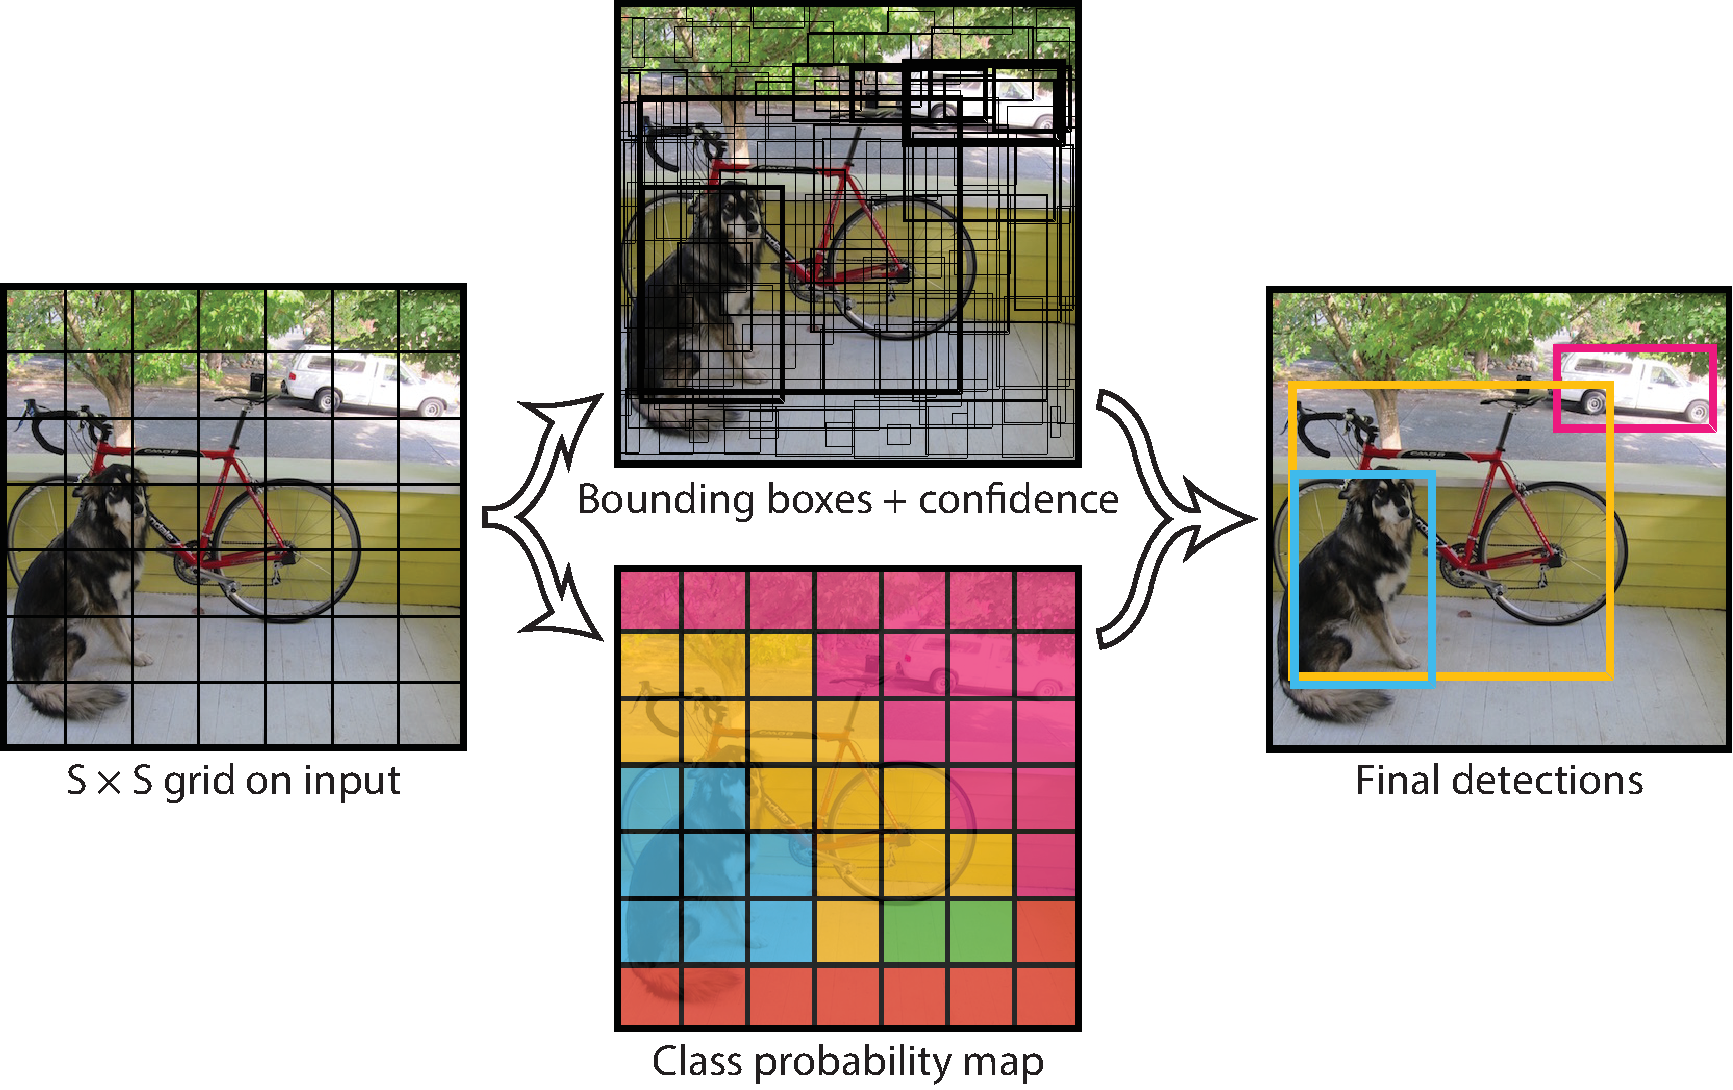
\includegraphics[scale=0.4,trim={0cm 5.6cm 21.5cm 3cm},clip]{images/dog.pdf}        
		};    
		\node(label) at (0,-1.8){\footnotesize Input Image};
	}
	\onslide<2-10>{
		\node(img) at (0,0.15){
			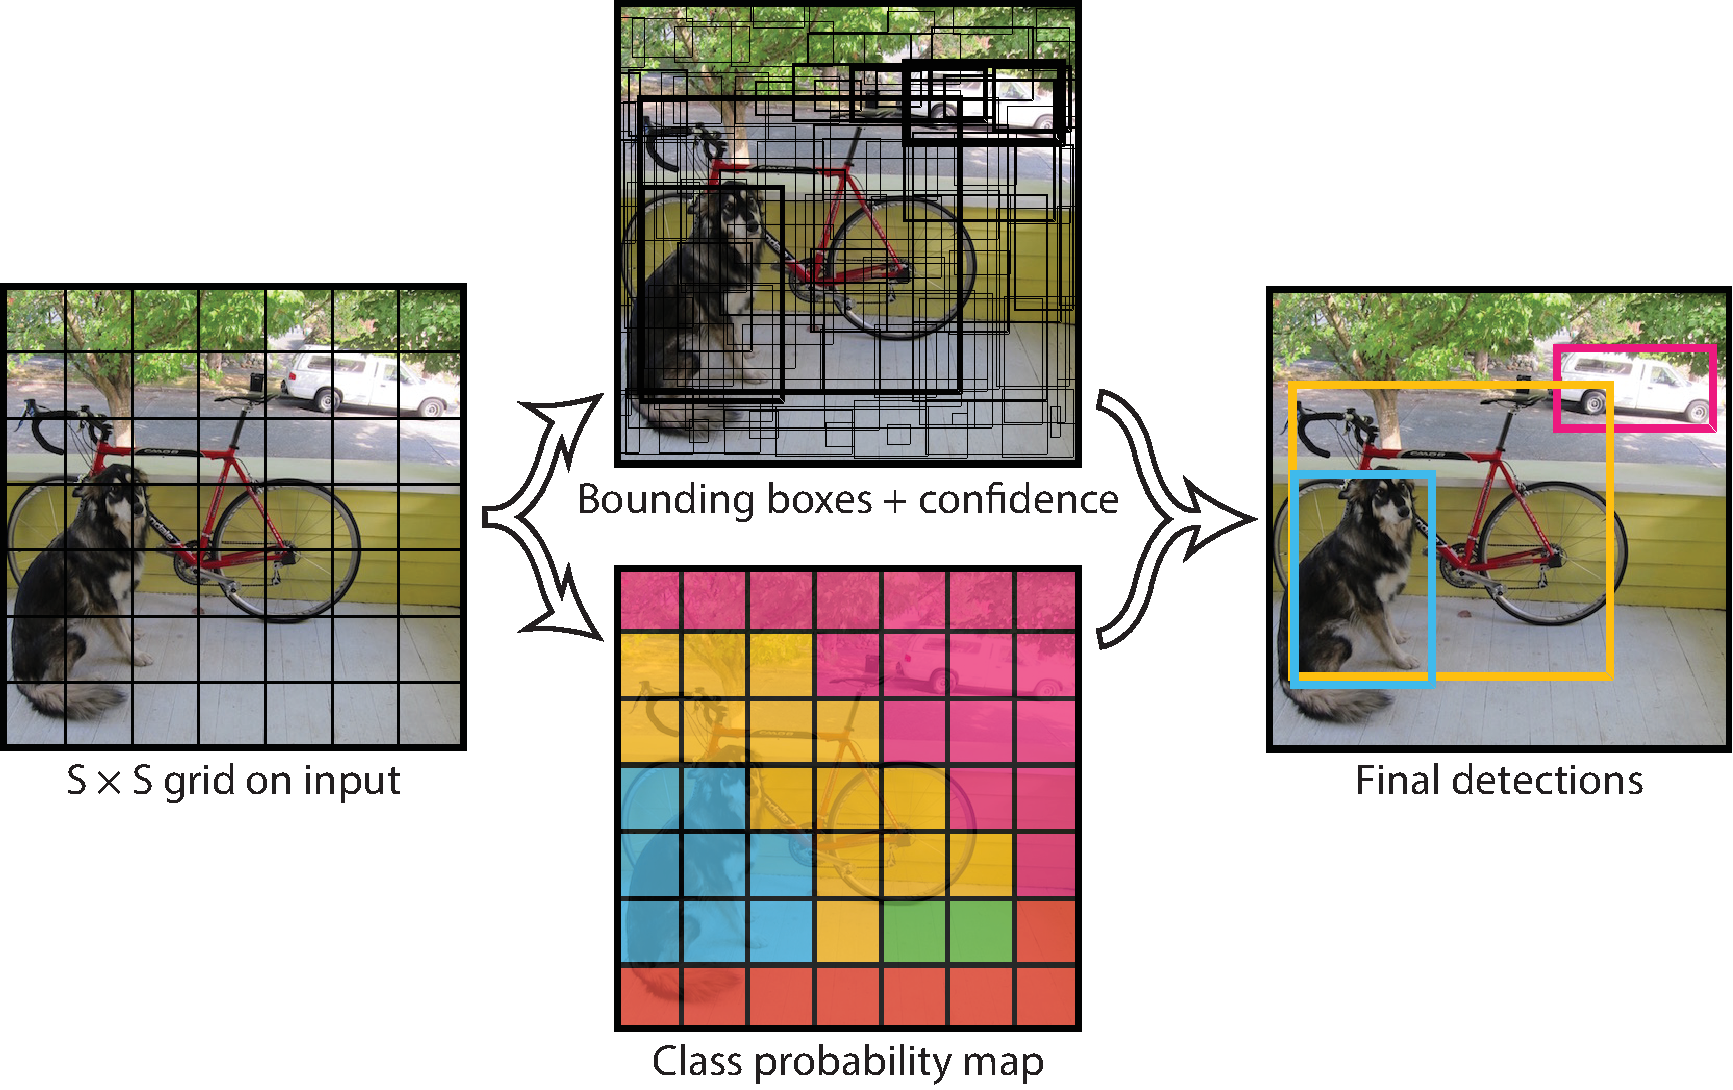
\includegraphics[scale=0.4,trim={0cm 4.5cm 21.2cm 4cm},clip]{images/dog.pdf}
		};
		\pgfmathsetmacro\x{-1.2}
		\pgfmathsetmacro\y{-0.45}
		\filldraw[fill=cyan!80, draw=cyan,opacity=0.5](\x,\y) rectangle (\x+0.48,\y+0.48);
	}
	\onslide<3-10>{
		\draw[line width=0.7mm,color=cyan] (-1.4,-0.9) rectangle (-0.5,0.6);  
	}

	\onslide<4-10>{
		\pgfmathsetmacro\x{0.6}
		\pgfmathsetmacro\y{-0.9}
		\filldraw[fill=green!70, draw=black,opacity=0.5](\x,\y) rectangle (\x+0.48,\y+0.48);
	}
	\onslide<5-10>{
		\draw[line width=0.2mm,color=green,dashed] (0.2,-1.2) rectangle (1.5,-0.12);  
	}
	\onslide<6-10>{
		\pgfmathsetmacro\x{-0.75}
		\pgfmathsetmacro\y{0}
		\filldraw[fill=yellow!70, draw=black,opacity=0.5](\x,\y) rectangle (\x+0.48,\y+0.48);
	}
	\onslide<7-10>{
		\draw[line width=0.1mm,color=yellow,line width=0.7mm] (-1.4,-0.8) rectangle (0.7,1.2);  
   
	}

	\onslide<8-10>{
		\pgfmathsetmacro\x{0.6}
		\pgfmathsetmacro\y{0.9}
		\filldraw[fill=magenta!70, draw=black,opacity=0.5](\x,\y) rectangle (\x+0.48,\y+0.48);
	}
	\onslide<9-10>{
		\draw[line width=0.1mm,color=magenta,line width=0.7mm] (0.3,0.8) rectangle (1.5,1.5); 

	}

	\onslide<10>{
		
		\pgfmathsetseed{1}
		\foreach \x in {-0.8,-0.5,...,0.8}{
			\foreach \y in {-0.8,-0.4,...,0.8}{
				\draw[red!50,dashed] (\x+rand,\y)rectangle (\x+rand,\y+rand);       
			}
		}     
		

		\draw[red,dashed] (0,0.15)rectangle (0.5,0.5);
		
		\node(label) at (0,-2.3){\footnotesize Bounding Boxes \& Confidence};
	}
	

	\onslide<11->{
		\node(img) at (0,1.2){
			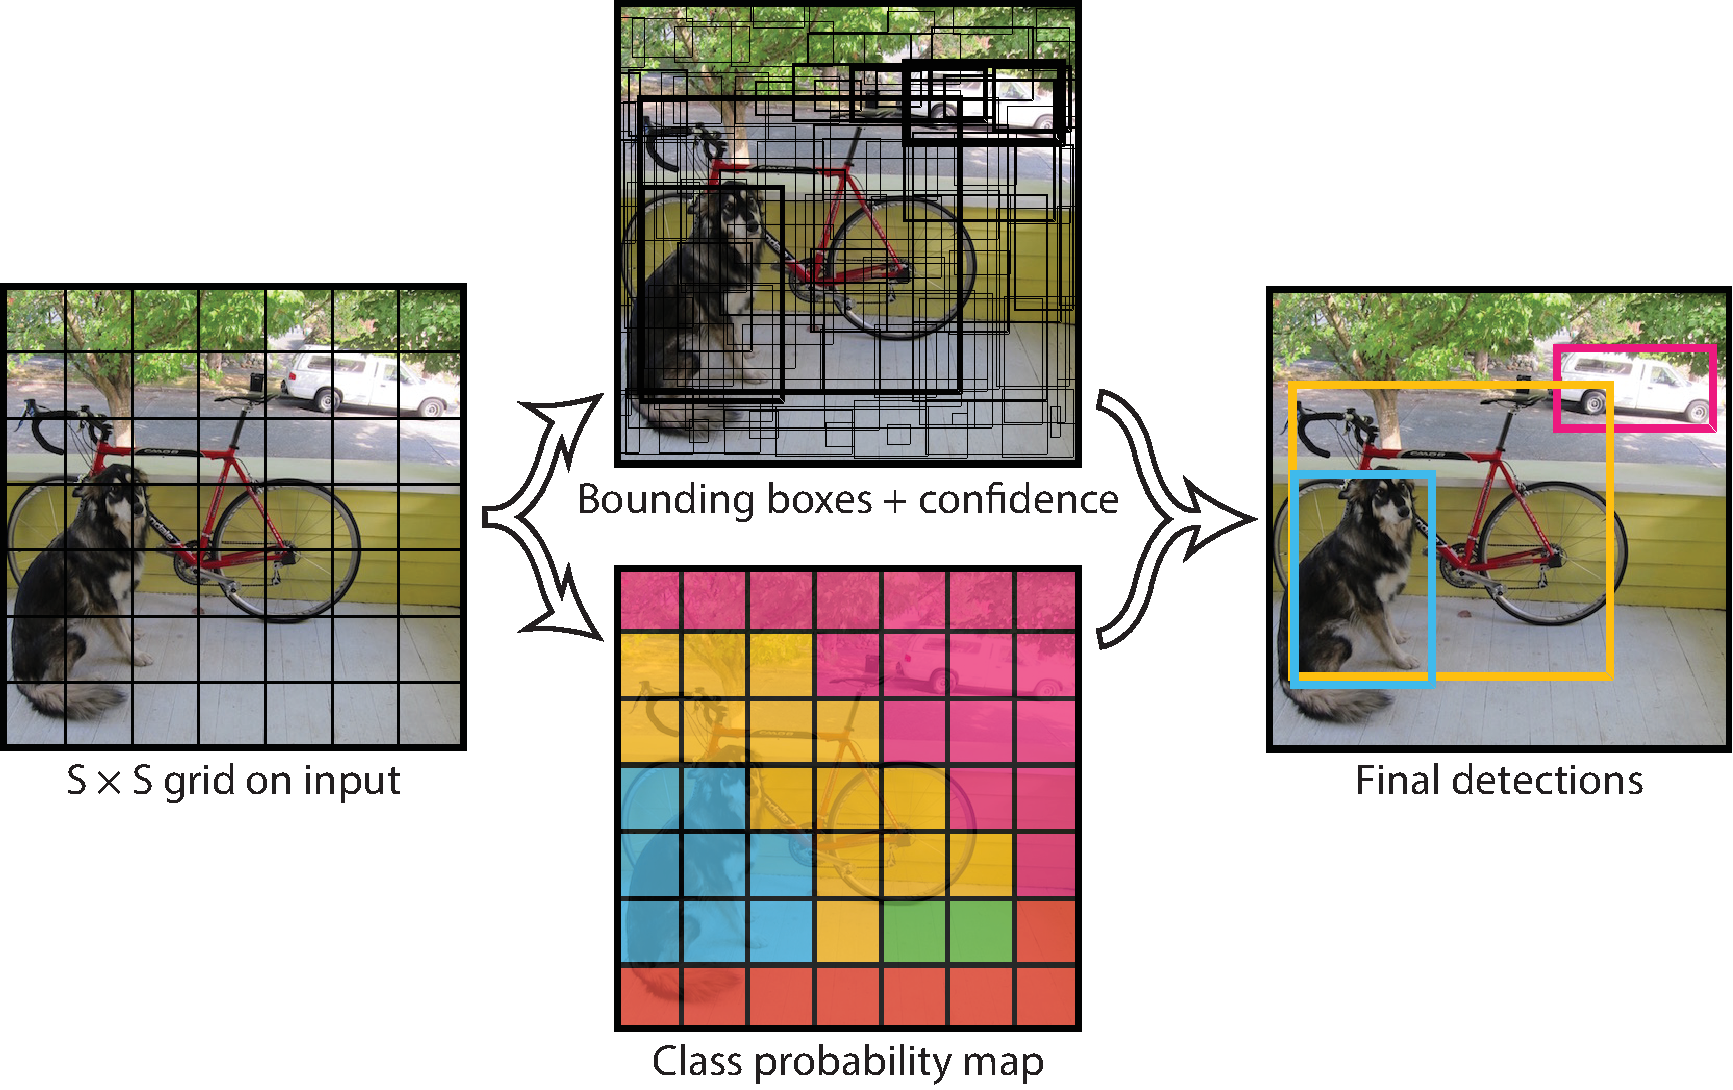
\includegraphics[scale=0.41,trim={21.5cm 5.6cm 0cm 0cm},clip]{images/dog.pdf}
		};
		%     \node(label) at (0,-2){\footnotesize Final Detection};
	}
\end{tikzpicture}

		\column{0.5\textwidth}
		\begin{itemize}
			\justifying
			\onslide<1->{\item How do we interpret this $S \times S \times (5+k)$ dimensional output?}
			\onslide<2->{\item For each cell, we are computing a bounding box, its confidence and the object in it}
			\onslide<11->{\item We then retain the most confident bounding boxes and the corresponding object label}
		\end{itemize}
	\end{columns}
\end{frame}

%%%%%%%%%%%%%%%%%%%%%%%%%%%%%%%%%%%%%%%%%%%%%%%%%%%%%%%%%%%%%%%%%%%%%%%%%%%%%%

\begin{frame}

	\begin{columns} 
		\column{0.5\textwidth}

		\begin{overlayarea}{\textwidth}{\textheight}      
			\begin{tikzpicture}
	\centering
	\onslide<1->{
		\pgfmathsetmacro\x{0}
		\pgfmathsetmacro\y{3}

		\draw (0,0+\y) grid[xstep=0.5,ystep=0.5] (5,0.5+\y);
		\node (w) at (0.25,\y+0.25) {\scriptsize $\hat{c}$};
		\node (h) at (0.75,\y+0.25) {\scriptsize $\hat{w}$};
		\node (x) at (1.25,\y+0.25) {\scriptsize $\hat{h}$};
		\node (y) at (1.75,\y+0.25) {\scriptsize $\hat{x}$};
		\node (pc) at (2.25,\y+0.25) {\scriptsize $\hat{y}$};
		\node (pd) at (2.75,\y+0.25) {\scriptsize $\hat{\ell_1}$};

		\node (w) at (3.25,\y+0.25) {\scriptsize $\hat{\ell_2}$};
		\node (h) at (3.75,\y+0.25) {$\cdot$};

		\node (w) at (4.25,\y+0.25) {$\cdot$};
		\node (h) at (4.75,\y+0.25) {\scriptsize $\hat{\ell_k}$};   

		\draw (0,0+\y)--(5,0+\y);

		\node(img) at (2.5,0){
			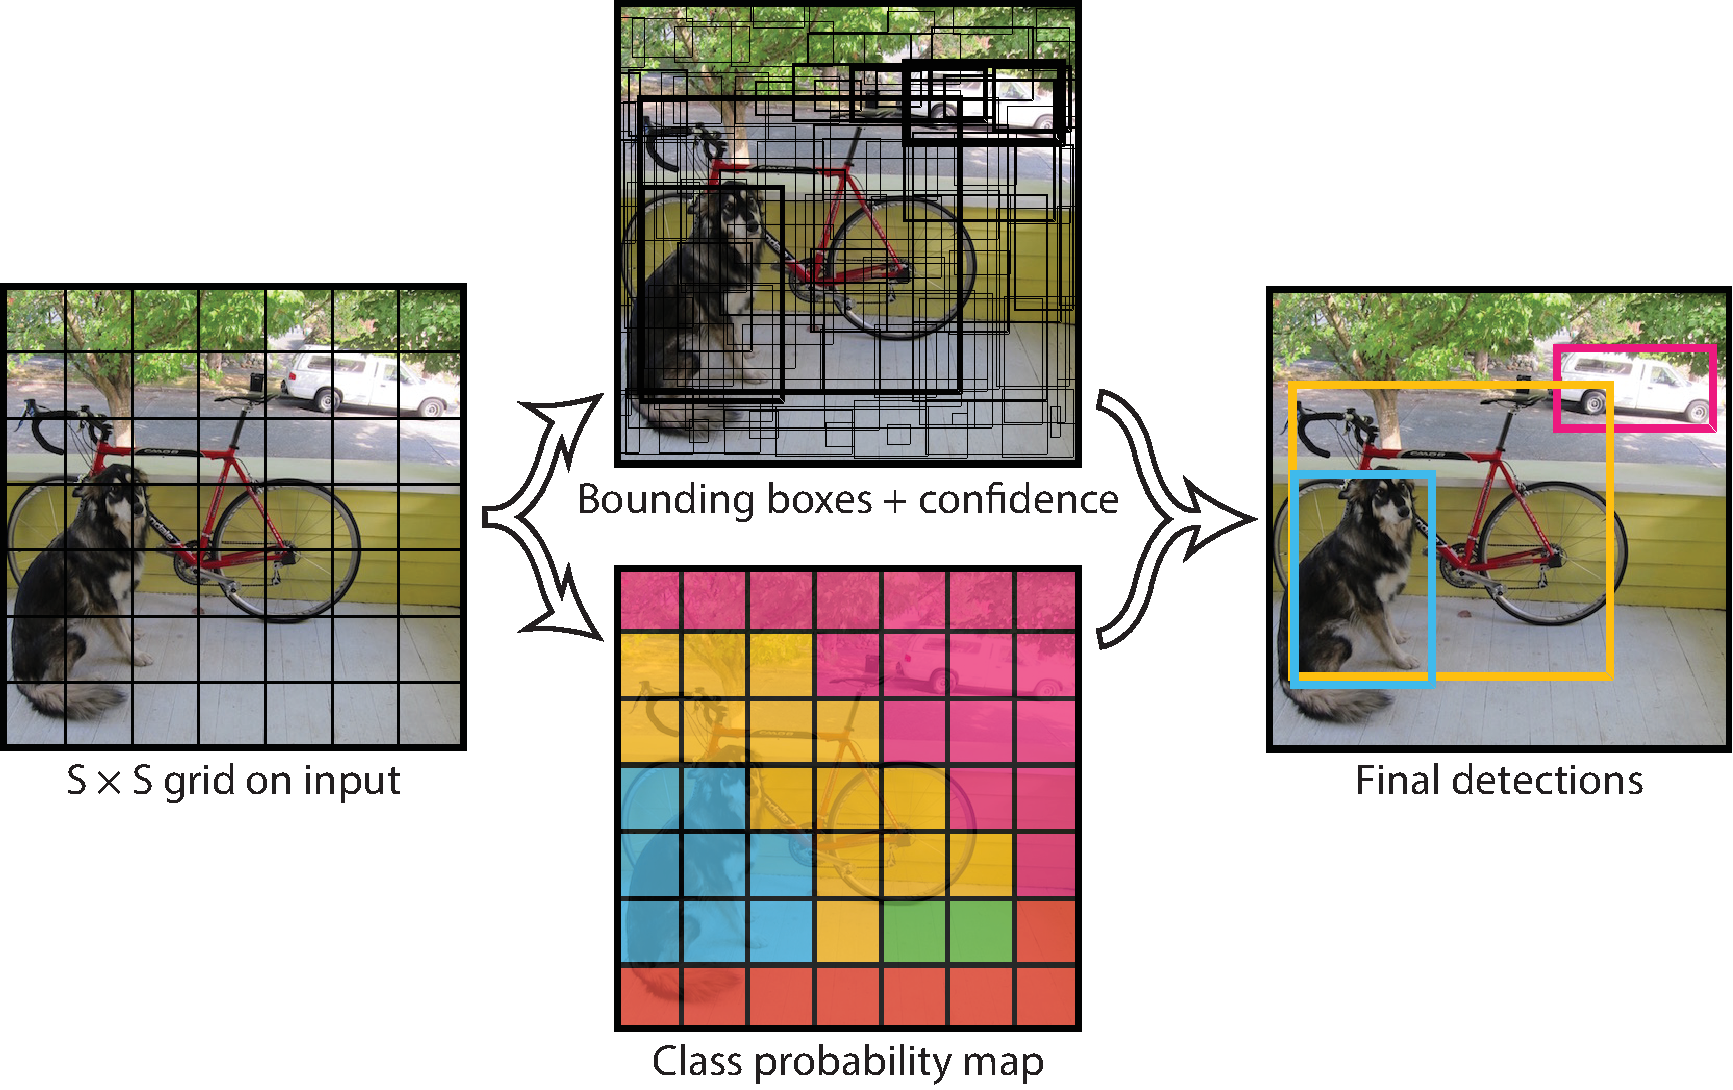
\includegraphics[scale=0.4,trim={0cm 4.5cm 21.2cm 4cm},clip]{images/dog.pdf}
		};

	}

	\onslide<2->{

		\pgfmathsetmacro\x{0}
		\pgfmathsetmacro\y{0.5}

		\node(img) at (2.5,0){
			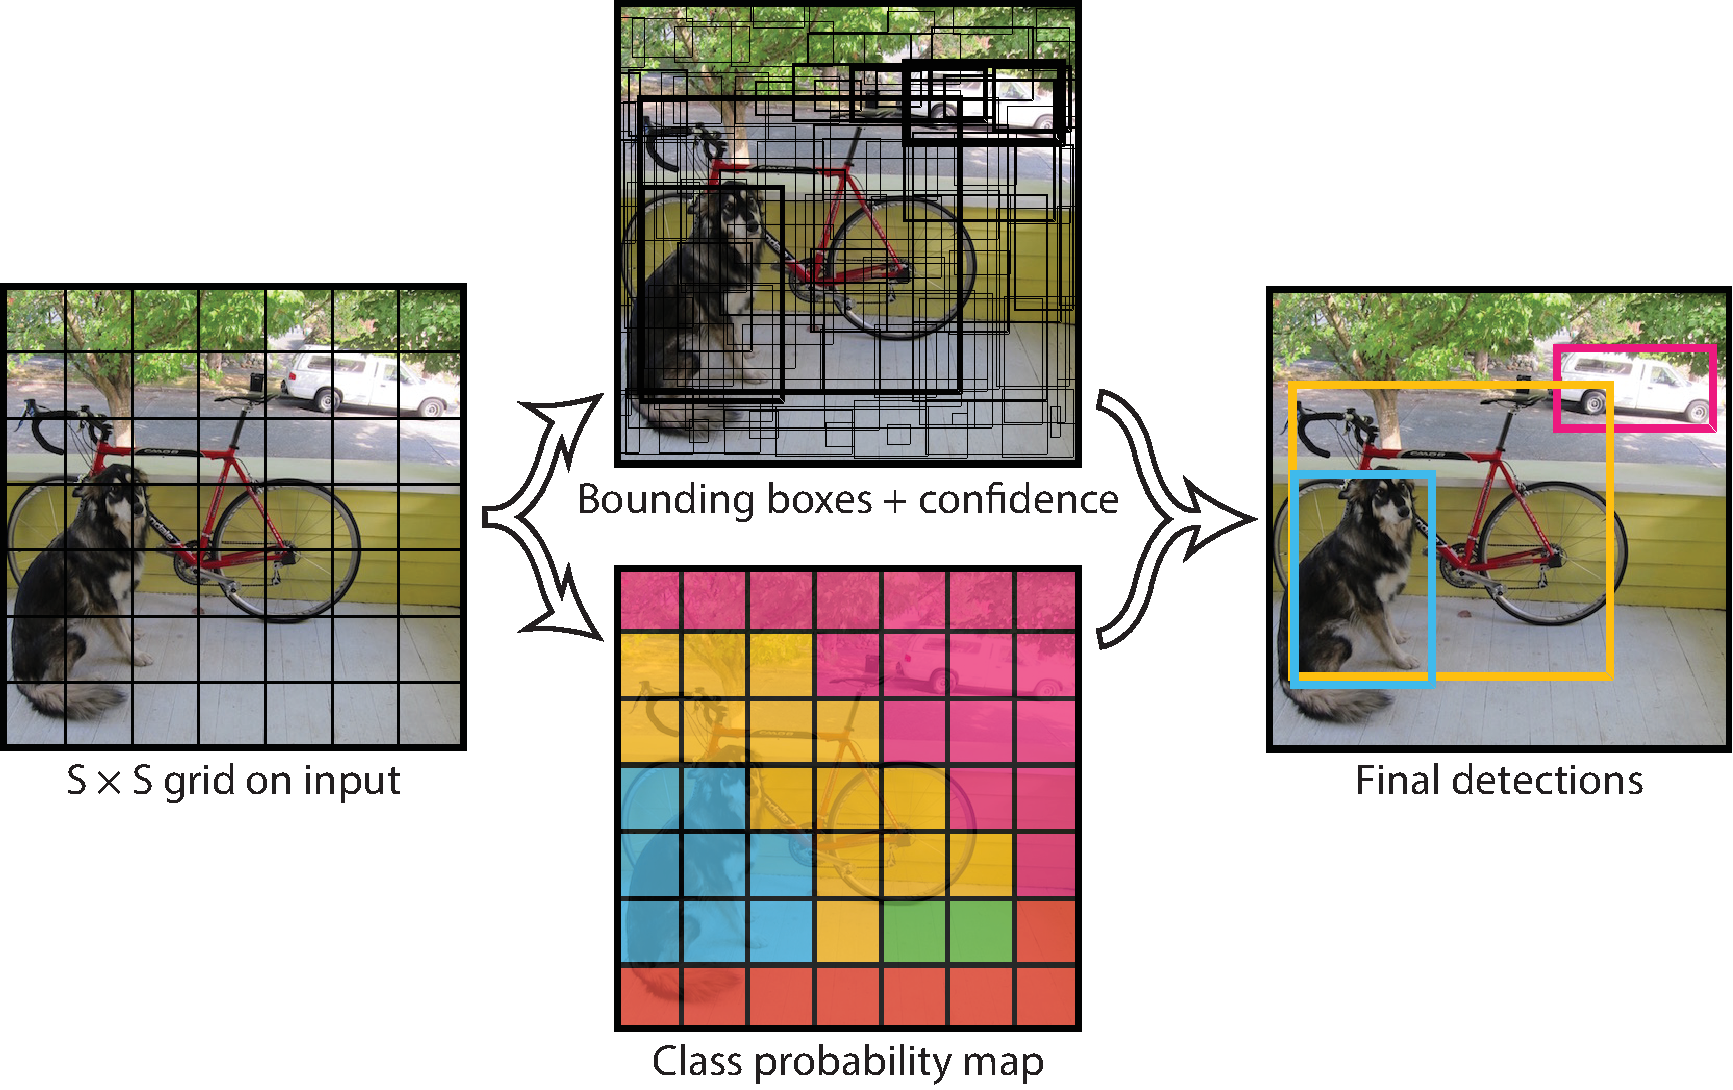
\includegraphics[scale=0.4,trim={0cm 4.5cm 21.2cm 4cm},clip]{images/dog.pdf}
		};
		
		\pgfmathsetmacro\x{1.3}
		\pgfmathsetmacro\y{-0.6}
		\filldraw[fill=cyan!30!white, draw=black,opacity=0.6](\x,\y) rectangle (\x+0.48,\y+0.48);
		
		\pgfmathsetmacro\x{0}
		\pgfmathsetmacro\y{2}
		\draw[line width=0.7mm,color=cyan] (\x+1,\y-3.3) rectangle (\x+2,\y-1.5);     
	}
	
	\only<5>{
		\filldraw[fill=green!40!white, draw=black](0,3) rectangle (0.5,3.5);    
		\node (w) at (0.25,3.25) {\scriptsize $c$};
	}

	\only<6>{
		\filldraw[fill=green!40!white, draw=black](0.5,3) rectangle (1,3.5);    
		\node (h) at (0.75,3.25) {\scriptsize $w$};
	}

	\only<7>{
		\filldraw[fill=green!40!white, draw=black](1,3) rectangle (1.5,3.5);    
		\node (x) at (1.25,3.25) {\scriptsize $h$};
	} 
	
	\only<8-9>{
		\filldraw[fill=green!40!white, draw=black](1.5,3) rectangle (2,3.5);    
		\node (y) at (1.75,3.25) {\scriptsize $x$};
		\filldraw[fill=green!40!white, draw=black](2,3) rectangle (2.5,3.5);    
		\node (x) at (2.25,3.25) {\scriptsize $y$};
	} 

	\onslide<10->{

		\filldraw[fill=green!40!white, draw=black](2.5,3) rectangle (5,3.5);
		\draw (0,3) grid[xstep=0.5,ystep=0.5] (5,3.5);
		\node (pd) at (2.75,4.25) {\scriptsize $P(cow)$};

		\node (w) at (3.25,2.75) {\scriptsize $P(dog)$};
		\node (h) at (3.75,3.25) {$\cdot$};

		\node (w) at (4.25,3.25) {$\cdot$};
		\node (h) at (4.75,3.75) {\scriptsize $P(truck)$};
	}   
	

	
\end{tikzpicture}

		\end{overlayarea}     
		\column{0.5\textwidth}
		\begin{overlayarea}{\textwidth}{\textheight}  
			%\scriptsize{   
			\begin{itemize}
				\justifying
				\onslide<1->{\item How do we train this network ?}
				\onslide<2->{\item Consider a cell such that the center of the true bonding box lies in it }
				\onslide<3->{\item The network is initialized randomly and it will predict some values for $c,w,h,x,y$ \& $\ell$}
				\onslide<4->{\item We can then compute the following losses}
				\only<8>{\item $(x-\hat{x})^2$
					%     \item       
				}
				\only<9>{\item $(y-\hat{y})^2$
					%     \item       
				}
				\only<6>{\item $(\sqrt{w}-\sqrt{\hat{w}})^2$
					%     \item       
				}
				\only<7>{\item $(\sqrt{h}-\sqrt{\hat{h}})^2$
					%     \item       
				}
				\only<5>{\item $(1-\hat{c})^2$
					%     \item       
				}
				\onslide<10->{\item $\sum_{i=1}^{k}(\ell_i-\hat{\ell_i})^2$
					%     \item       
				}
				\onslide<11->{\item And train the network to minimize the sum of these losses}
			\end{itemize}
			% }
		\end{overlayarea}
	\end{columns}
\end{frame}

%%%%%%%%%%%%%%%%%%%%%%%%%%%%%%%%%%%%%%%%%%%%%%%%%%%%%%%%%%%%%%%%%%%%%%%%%%%%%%

\begin{frame}
	\begin{overlayarea}{\textwidth}{\textheight}  
		\begin{columns}
			\column{0.5\textwidth}
			\begin{tikzpicture}
	\vspace*{0.5cm}
	\centering
	\onslide<1->{
		\pgfmathsetmacro\x{0}
		\pgfmathsetmacro\y{3}

		\draw (0,0+\y) grid[xstep=0.5,ystep=0.5] (5,0.5+\y);
		\node (w) at (0.25,\y+0.25) {\scriptsize $\hat{c}$};
		\node (h) at (0.75,\y+0.25) {\scriptsize $\hat{w}$};
		\node (x) at (1.25,\y+0.25) {\scriptsize $\hat{h}$};
		\node (y) at (1.75,\y+0.25) {\scriptsize $\hat{x}$};
		\node (pc) at (2.25,\y+0.25) {\scriptsize $\hat{y}$};
		\node (pd) at (2.75,\y+0.25) {\scriptsize $\hat{\ell_1}$};

		\node (w) at (3.25,\y+0.25) {\scriptsize $\hat{\ell_2}$};
		\node (h) at (3.75,\y+0.25) {$\cdot$};

		\node (w) at (4.25,\y+0.25) {$\cdot$};
		\node (h) at (4.75,\y+0.25) {\scriptsize $\hat{\ell_k}$};   

		\draw (0,0+\y)--(5,0+\y);

		\node(img) at (2.5,0){
			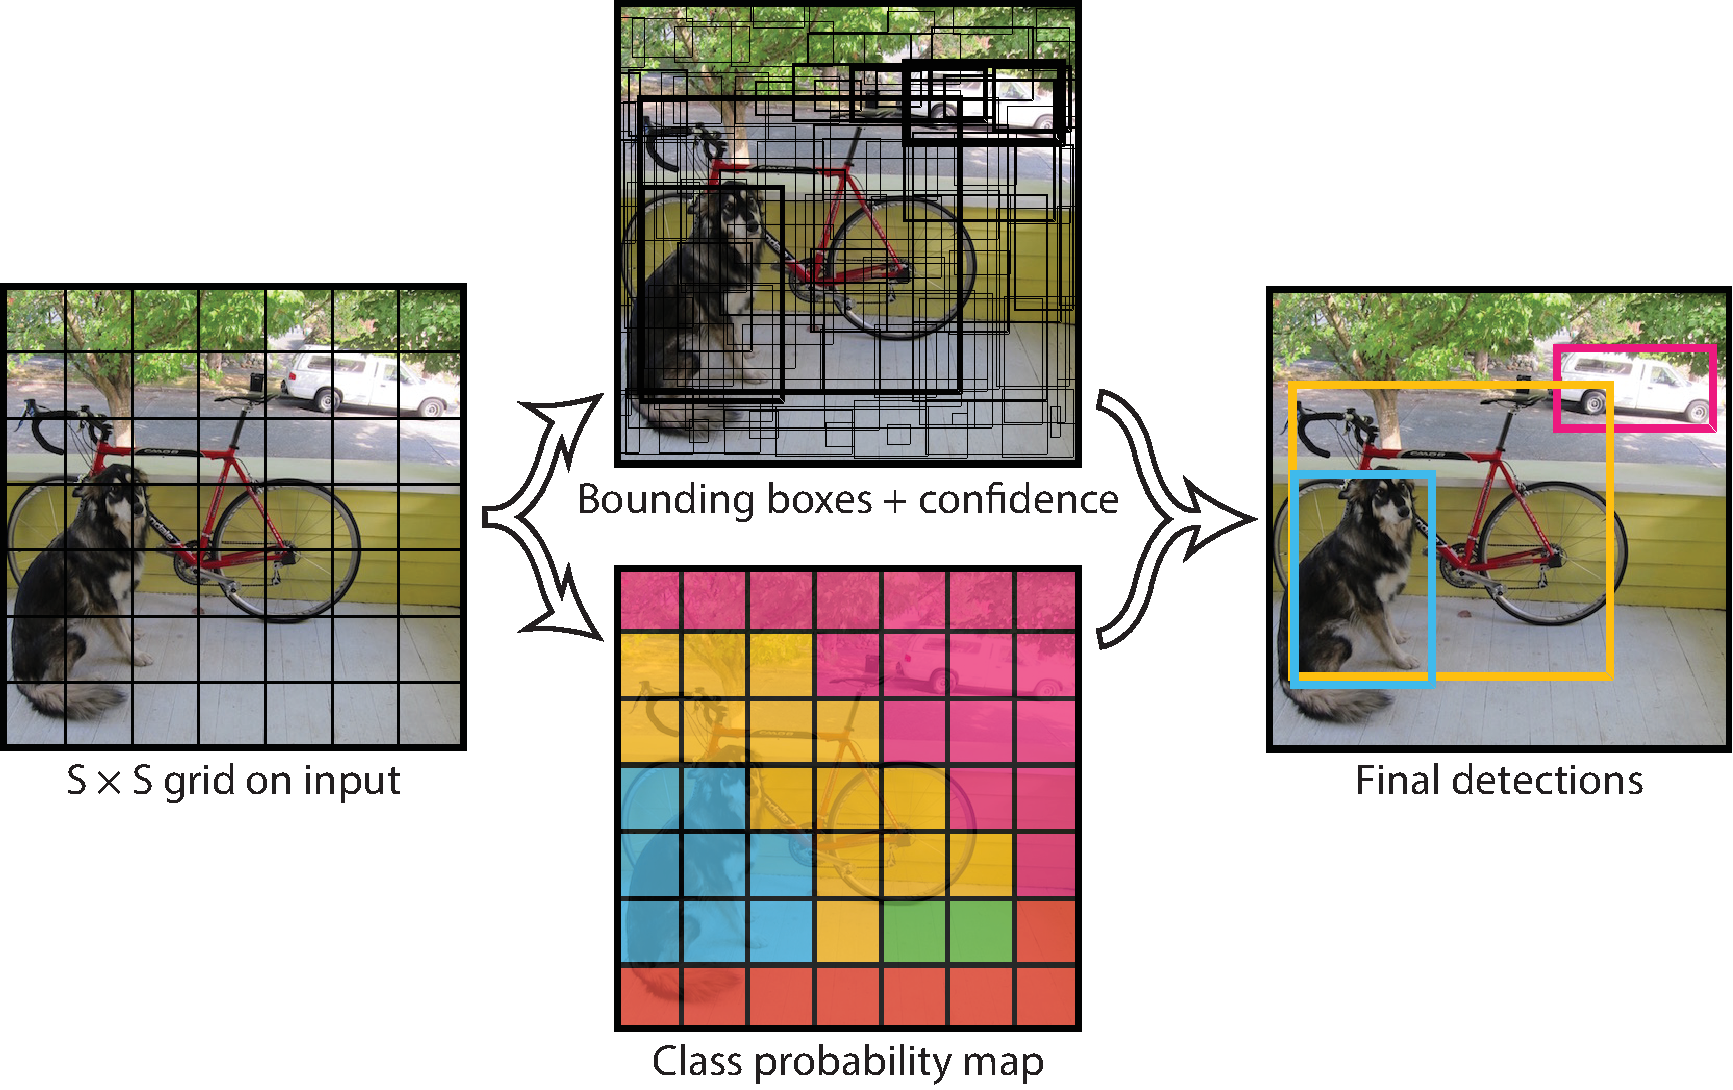
\includegraphics[scale=0.4,trim={0cm 4.5cm 21.2cm 4cm},clip]{images/dog.pdf}
		};

		\pgfmathsetmacro\x{0.6+2.5}
		\pgfmathsetmacro\y{-1.05}
		\filldraw[fill=green!50!white, draw=black,opacity=0.6](\x,\y) rectangle (\x+0.48,\y+0.48);
		\draw[line width=0.1mm,color=green] (0.5+2.3,-1.3) rectangle (1.3+2.5,-0.1);    
	}

	\onslide<2->{
		\pgfmathsetmacro\x{0}
		\pgfmathsetmacro\y{3}
		\filldraw[color=gray!70!white](0.5,0+\y) rectangle (5,0.5+\y);
		%\filldraw[color=gray!70!white](2.5,0+\y) rectangle (5,0.5+\y);
		\draw (0,0+\y) grid[xstep=0.5,ystep=0.5] (5,0.5+\y);
	}

	
	
\end{tikzpicture}

			\column{0.5\textwidth}
			\begin{itemize}
				\justifying
				\onslide<1->{\item Now consider a grid which does not contain any object}
				\onslide<2->{\item For this grid we do not care about the predictions $w,h,x,y$ \& $\ell$}     
				\onslide<3->{\item But we want the confidence to be low}
				\onslide<4->{\item So we minimize only the following loss
					\begin{equation*}
						(0 - \hat{c})^2
					\end{equation*}
				}
			\end{itemize}
		\end{columns}
	\end{overlayarea}
\end{frame}

%%%%%%%%%%%%%%%%%%%%%%%%%%%%%%%%%%%%%%%%%%%%%%%%%%%%%%%%%%%%%%%%%%%%%%%%%%%%%%

\begin{frame}
	\begin{table}
		\begin{tabular}{ccc}
			\hline
			\textbf{Method}           & \textbf{Pascal 2007 mAP} & \textbf{Speed}                         \\
			\hline
			\onslide<1->{DPM v5}      & \onslide<1->{33.7}       & \onslide<1->{0.07 FPS | 14 sec/ image} \\ 
			\onslide<2->{RCNN}        & \onslide<2->{66.0}       & \onslide<2->{0.05 FPS | 20 sec/ image} \\ 
			\onslide<3->{Fast RCNN}   & \onslide<3->{70.0}       & \onslide<3->{0.5 FPS | 2 sec/ image}   \\ 
			\onslide<4->{Faster RCNN} & \onslide<4->{73.2}       & \onslide<4->{7 FPS | 140 msec/ image}  \\ 
			\onslide<5->{YOLO}        & \onslide<5->{69.0}       & \onslide<5->{45 FPS | 22 msec/ image}  \\ 
			\hline
		\end{tabular}
	\end{table}
	
\end{frame}
